
\begin{figure}[!h]
    \centering
        %Prima riga
        \begin{subfigure}{0.48\textwidth} %Controllo della posizione in orizzontale
            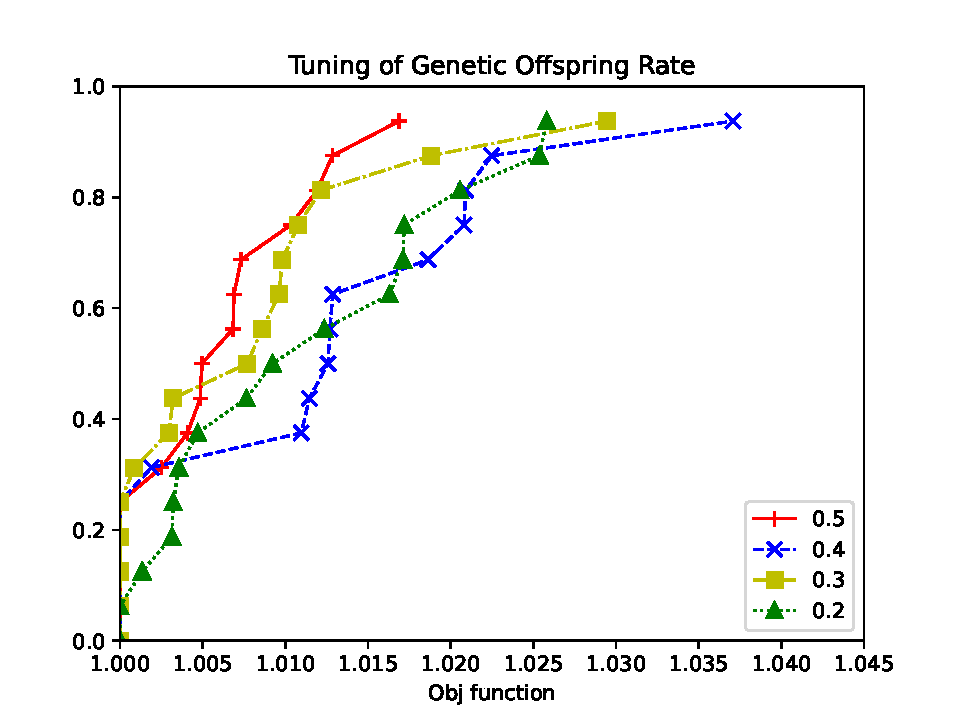
\includegraphics[scale=0.45]{images/genoff.pdf} 
            \caption{Tuning of Offspring Rate}
            \label{fig:genoff}
        \end{subfigure}
        \begin{subfigure}{0.48\textwidth}
            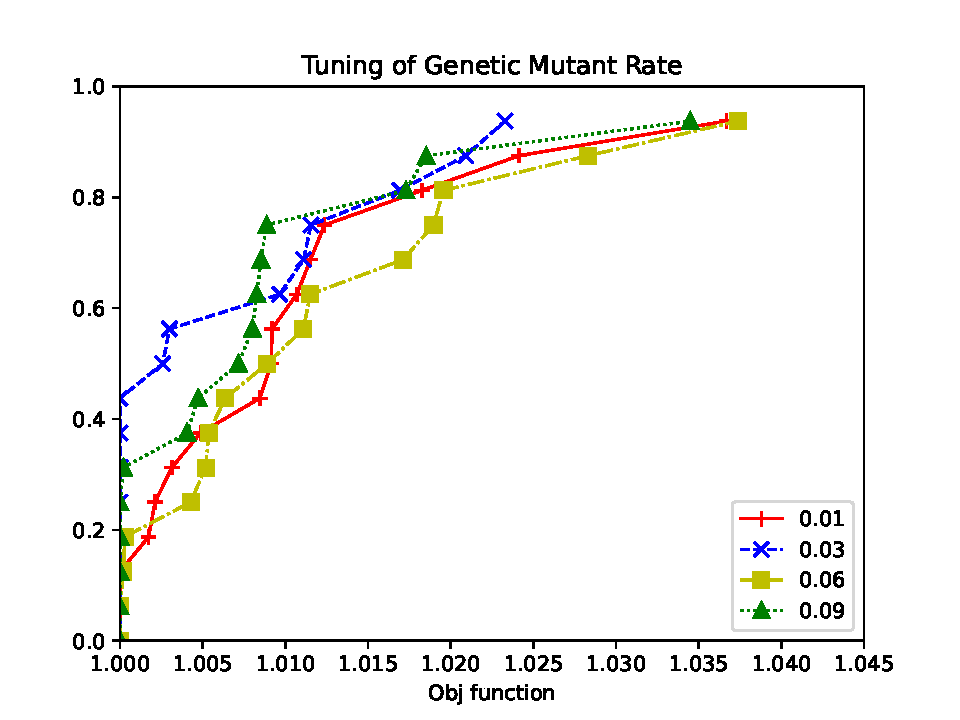
\includegraphics[scale=0.45]{images/genmut.pdf}
            \caption{Tuning of Mutant Rate}
            \label{fig:genmut}
        \end{subfigure}
    \caption{Tuning of the Genetic algorithm}
    \end{figure}

\subsection{Tuning of Genetic}

The most important parameters in the Genetic algorithm are the \textit{Offspring Rate} and the \textit{Mutant Rate}.

The \textit{Offspring Rate} determines the size of the new offspring generation based over a percentage of the size of the actual generation. This value changes the rate of finding possible better chromosomes, slowling or speeding up the process of natural selection.

In Figure \ref{fig:genoff} can be seen that the values that compete the most are 0.5 and 0.3, but in the final implementation of the algorithm we chose \textit{Offspring Rate} = 0.5 since it performed better in the most cases.


The \textit{Mutant Rate} is tuned to add some well weighted randomness to the algorithm. Too many mutants can lead to worse possibilities of improvement, but a mutant is essential to assert a possibility of escapism from a possible local optima. 

We tested the range [0.1,0.9] to keep the probability of adding a mutant really low, and we can see in Figure \ref{fig:genmut} that both 0.03 and 0.09 compete really well, but we chose to use a \textit{Mutant Rate} = 0.09.



